\documentclass[10pt,twocolumn]{article}

\usepackage[small,compact]{titlesec} %http://gurmeet.net/computer-science/latex-tips-n-tricks-for-conference-papers/
\usepackage{microtype} % Make the font and alignment look cleaner
\usepackage{graphicx}

% For \overset, etc.
\usepackage{amsmath}
\usepackage{cancel}

%%%%%%%%%%%%%%%%%%%%%%%%%%%%%% Margins
\setlength{\columnsep}{0.25in}
\usepackage[top=0.8in,bottom=0.8in,left=0.5in,right=0.5in]{geometry}




%==================================================================================================
%   MATH MACROS
\newcommand{\mabs}[1]{\ensuremath{  \left| #1 \right|  }}
\newcommand{\argmax}[2]{\ensuremath{   \underset{#1}{\operatorname{argmax}} \left\{ #2 \right\}  }} 

\newcommand{\prb}[1]{\ensuremath{  \mathrm{Pr}\left\{ #1 \right\}  }}
\newcommand{\Elin}[1]{\ensuremath{     \mathrm{E}\left[ #1 \right]   }}

\newcommand{\tridefeq}{\ensuremath{  \,{\overset{\triangle}{=}}\;   }}

\newcommand{\normrv}[2]{\ensuremath{          \mathcal{N}\left(#1,#2\right)    }}

\newcommand{\ind}[1]{\ensuremath{  \pmb{\mathtt{1}}\left\{ #1 \right\}  }}

%==================================================================================================

\begin{document}


 \twocolumn[%
 \centerline{\Large \bf Bayesian Skill Ranking} %% Paper title

 \medskip

 \centerline{\bf Leland Chen, Joseph Huang, Ryan Thompson}      %% Author name(s)
 \centerline{\today}

 \bigskip
 ]

% ==============================================================================
% ==============================================================================

\section{Introduction}

	In this paper, we examine professional basketball games in the context of Bayesian Skill Ranking. By modeling every possession as a data point parameterized by a number of points scored and a binary-valued vector of players on the court, we hope to infer player skill levels in six abilities - one-point, two-point, and three-point offense and defense. There are many existing rating systems, but most are designed for single-player games with simple binary outcomes. In order to successfully model basketball outcomes, we built a network with a likelihood function that can be maximized via Expectation-Maximization. We model our main variables with both a logit and probit function, which we use to estimate each player's skill rankings.

% ==============================================================================
% ==============================================================================

\section{Related Work}

For head-to-head competitions (Player A vs. Player B) with binary outcomes (Player A Wins, Player A Loses), there exist many well-understood techniques for compressing player performances into a single skill parameter.
ELO~\cite{elo1978rating} is the most widespread such ranking system.
ELO was initially designed around a probit model that determined probability of Player A defeating Player B as a function of the difference of their skill ranking. However, the model was soon changed to the better-performing logit Bradley-Terry model, as suggested originally by~\cite{bradley1952rank}.

Other ranking systems, such as Glicko~\cite{glickman1999parameter}, model the probability of winning as both a logit and probit function, which are very similar in distribution but have different convergence properties and perform differently at the tails of the distributions.

More recent developments in ranking systems deal with team behavior and performance, and Bayesian networks where skill influences performance, and performance variables are combined to determine winning probabilities. TrueSkill ~\cite{herbrich2007trueskilltm}~ is used for Halo rankings in both individual and cooperative modes, but it only uses Gaussian priors for skill and performance. Whole-History Rating ~\cite{coulom2008whole} focuses on varying skill parameters over time, to account for players improving with practice and declining with age.

The Elo rating system is used for calculating relative skill levels of players in two-player games, but has been adapted to team sports like soccer, football, basketball, and baseball. The performance of players/teams is inferred from wins, losses, and draws against other players/teams, while depending on the ratings of the opponent and the results scored against them. (Elo also has some mathetmatical issues of that have been addressed through different means). Elo only considers the final score, which is not always indicative of how competitive the game was, and when used for teams, does not consider the players individually. Therefore, our intent is to build a more sophisticated model that determines 6 different skills (3 on offensive and 3 on defense) for each player using Bayesian Networks. By doing so, we can make better inferences on how well these sets of players contribute as a team on each possession and how likely they are to score 0, 1, 2, or 3 points per possession against their opponent. 

Basketball also brings more key challenges to the field of Bayesian Skill estimation.
\begin{itemize}
\item Results are not binary Win/Lose outcomes - or at least it is nearly impossible to distinguish between players abilities when only examining the final result of a game.
\item Results are influenced by the skill differential of more than two players.
\item A player's skill level is at least two parameters - offense and defense.
\end{itemize}



% ==============================================================================
% ==============================================================================

\section{Method}
\subsection{Traditional Networks}

We model the result of each possession as an independent and identically distributed random variable, \emph{Result}.
An NBA roster has 12 players, but only five of them are on the court for a given team during any single possession.

To reduce noise, we ignore ``garbage time" possessions. To simplify the model we will only consider possessions in the first half of games, or in the case of games that go to overtime, the entire game. This ensures that we take a lot of the gamesmanship and coaching strategy out of the data - we won't have to deal with starters resting or bench players playing a lot of minutes in a blowout.

We begin with a very basic model that follows traditional ``skill ranking" in the sense that each player has an unobserved (or parameterized) skill that has some distribution, and using inference (or parameter estimation) we can determine the value of each player's skill.
In this network, we decided each player would have a hidden offensive and defensive skill value, shared across possessions:
\begin{center}
	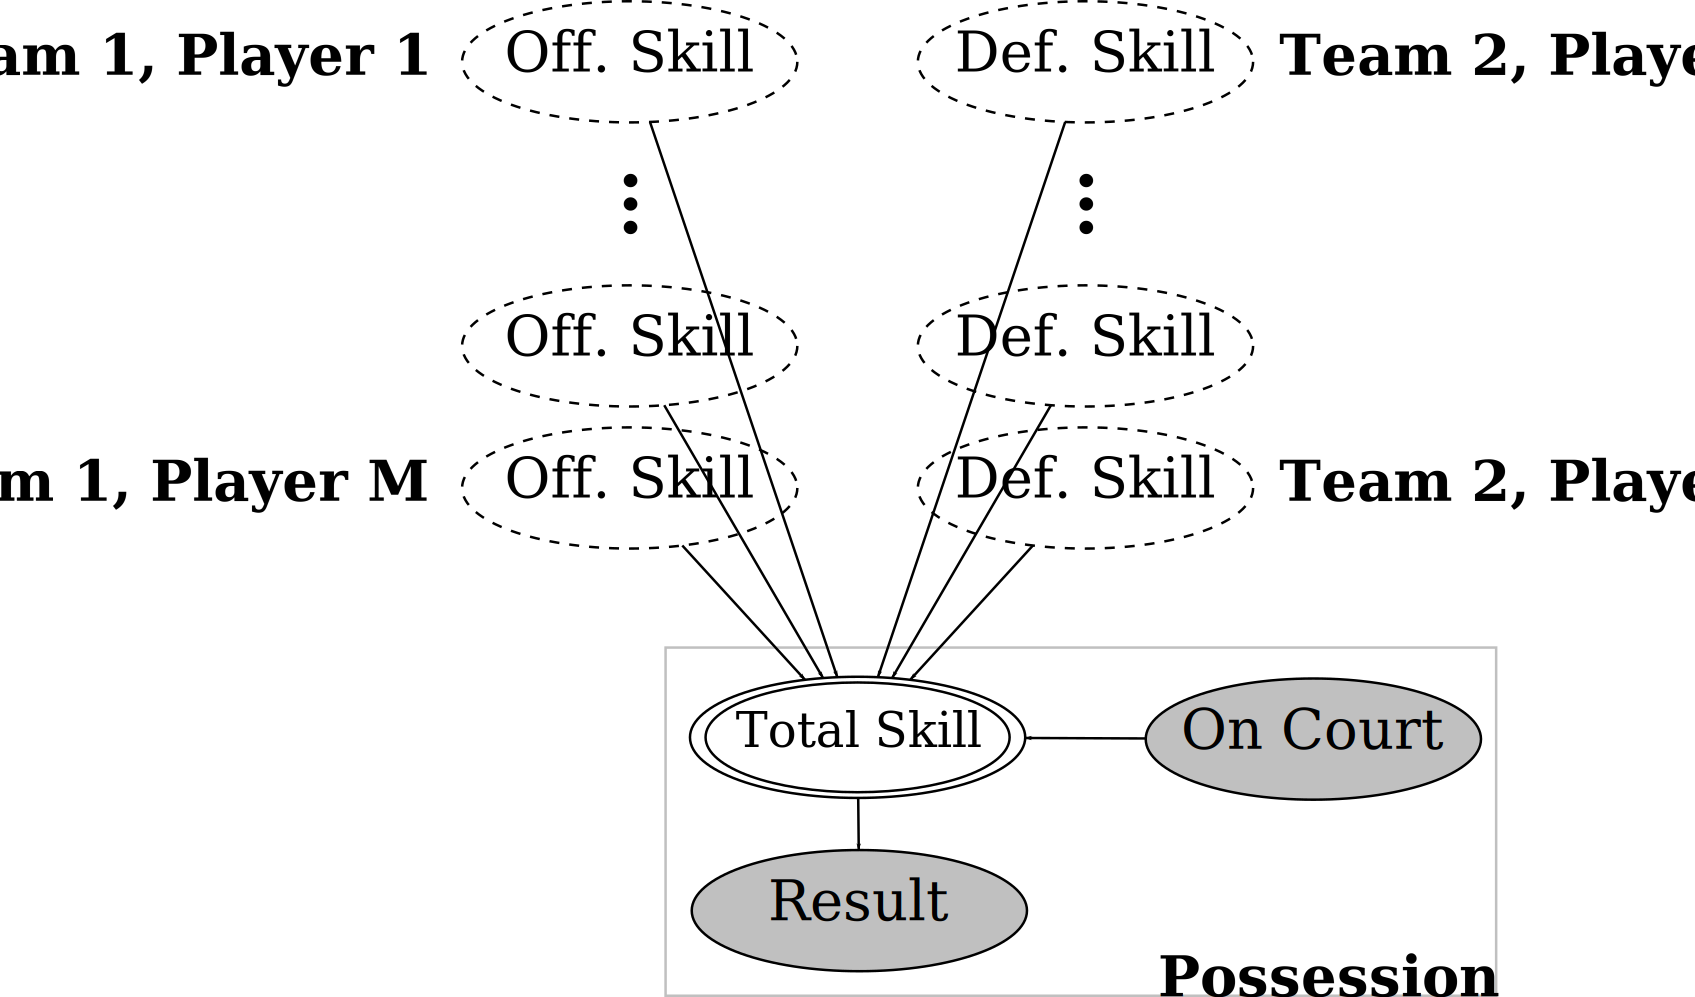
\includegraphics[width=0.90\linewidth]{figures/network}
\end{center}
These skills would contribute deterministically in some way to an ``effective'' total skill differential between the two teams, and then the \emph{Result} variable would be one of four outcomes:
\begin{itemize}
\item $R=0$ Offensive Team Scores nothing, change of possession (e.g. turnover, defensive rebound, etc.)
\item $R=1$ Offensive Team Scores 1 point
\item $R=2$ Offensive Team Scores 2 points
\item $R=3$ Offensive Team Scores 3 points
\end{itemize}

Note: We are ignoring the rare 4 point plays. 

The \emph{On Court} random variable "multiplexes" between those players that are on the court and those that are not.

% ==============================================================================
\subsection{Issues}
\label{sec:badnetwork}
These traditional models~\cite{herbrich2007trueskilltm} have difficulty capturing the proper causalities when Results can have multinomial-valued outcomes.
For example, regardless of the parameterization of the \emph{Results} CPD, both $\prb{ R = 2}$ and $\prb{R= 3}$ would depend on the same skills of the same players.
The relative distribution of outcomes $\prb{R = 2}$ vs. $\prb{R = 3}$ would be shared across all ``units" (i.e. all combinations of \emph{On Court} assignments).

In reality, a team that scores $R=3$ half the time and $R=1$ half the time is just as good as a team that scores $R=2$ all the time.
However, any traditional Win/Lose model will unfairly penalize the likelihood of one of these teams over the other and leads to under-fitting.
This might suggest that we have a random variable that represents $\Elin{\textrm{points scored}}$, but this doesn't pass the clarity test.

Secondly, there is a lot of value in being able to compare with the state-of-the-art in the Win/Lose based Bayesian Skill Ranking literature.
Specifically, there is common debate over logistic vs. Gaussian skill/performance distributions and we wish to be sensitive to that conversation in this project.
Having a multinomial outcome makes it difficult to directly compare logistic vs. Gaussian in the standard skill/performance framework because there is no consensus in the literature about how to extend these models just to support ties~\cite{hunter2004mm}, let alone general multinomial outcomes. This is part of our rationale for designing a network with a modular framework for different density functions.

% ==============================================================================
\subsection{Proposed Network}
\label{sec:goodnetwork}

To address some of the shortcomings discussed in {\bf Section~\ref{sec:badnetwork}}, we propose the following:
\begin{center}
	
\includegraphics[width=1.05\linewidth]{figures/newnetwork}
\end{center}

In this network, each player is represented by three skill parameters:
\begin{enumerate}
\item Skill 1: Ability to score (or defend against) one-point opportunities
\item Skill 2: Ability to score (or defend against) two-point opportunities
\item Skill 3: Ability to score (or defend against) three-point opportunities
\end{enumerate}

For notational convenience, let
\[
A\left(\mathrm{Skills}\right) \tridefeq \sum_i  \left( \textrm{Off. Team, Player i Off. Skill } k \right) * C_i
%\quad, \quad \quad
\]%
\[
B\left(\mathrm{Skills}\right) \tridefeq  \sum_i \left(  \textrm{Def. Team, Player i Def. Skill } k \right) * C_i
\]%
where
\[
C_i = binary value indicating whether player i is on-court
\]%

On each possession, there are three binary hidden random variables defined by a probability function with parameters that we will learn. In particular, each of the ``Win'' random variables depends on the corresponding skills of players on court as input (which are learned):
\begin{enumerate}
\item \emph{Win 1}: True if there was a {\bf guaranteed opportunity} to score one point at some point during the possession.
\item \emph{Win 2}: True if there was a {\bf guaranteed opportunity} to score two points at some point during the possession.
\item \emph{Win 3}: True if there was a {\bf guaranteed opportunity} to score three points at some point during the possession.
\end{enumerate}
Note: The term ``opportunity'' is not intended in the typical basketball sense, where it often means ``the opportunity to take a shot''.


Each of the \emph{Win k} events has a CPD parameterized by $\vec \theta_k$ (whose values we will learn during training), which depends on the skills of the players.
In the basic model of player skills, the skill of a five-man team is the sum of the skills of its players.

For example, the Bradley-Terry model corresponds to:
\[
\prb{\mathrm{Win}_k = \mathbf{True} \mid \mathrm{Skills} } = \frac{ A\left(\mathrm{Skills}\right) } { A\left(\mathrm{Skills}\right) + B\left(\mathrm{Skills}\right) }
\]%
Alternatively, the Thurstone Case V model corresponds to:
\[
\prb{\mathrm{Win}_k = \mathbf{True} \mid \mathrm{Skills} } = \Phi\left( A - B \right)
\]%
The logit (Bradley-Terry) and probit (Thurstone Case V) are the main Binary Response Models used throughout the history of the skill ranking literature~\cite{elo1978rating,glickman1999parameter,herbrich2007trueskilltm,coulom2008whole}.

However, the power of this Bayesian Network construction is that any Binary Response Model can be plugged in modularly.
One can easily compare the performance of Cauchy~\cite{franklinPolisciWiscEduMLELec07p4up}, Log-Log~and~Complementary Log-Log~\cite{long1997regression}, Scobit~\cite{nagler1994scobit}, etc. without changing the network or the core inference algorithm.

For notational convenience, we will write $W_k = w_k^1$ for $\mathrm{Win}_k = \mathbf{True}$, and $W_k = w_k^0$ when {\bf False}.

To understand the relationship between $\left\{Win\right\}$ and $Result$, let's go through an example.
Imagine that for a particular five-man unit, the $\theta$ are known and the resulting probabilities are:
\begin{align*}
\prb{W_1=w_1^1} = 5\% \quad&, \quad\quad \prb{W_1=w_1^0} = 95\%
\\
\prb{W_2=w_2^1} = 35\% \quad&, \quad\quad \prb{W_2=w_2^0} = 65\%
\\
\prb{W_3=w_3^1} = 10\% \quad&, \quad\quad \prb{W_3=w_3^0} = 90\%
\end{align*}%
This means, on each possession
\begin{itemize}
\item the offensive team has a $10\%$ probability of scoring 3 points (i.e. $R=r^3$ with 10\% probability)
\item the offensive team has a $\left(100\% - 10\%\right) \times 35\%$ probability of scoring 2 points (i.e. $\prb{R=r^2}=31.50\%$)
\item the offensive team has a $90\% \times 65\% \times 5\%$ probability of scoring 1 point (i.e. $\prb{R=r^1}=2.925\%$)
\item the offensive team has a $55.575\%$ chance of scoring 0 points
\end{itemize}

Essentially, \emph{Result} simply selects the highest-scoring decision available during the possession.
If \emph{Win 3} is true, \emph{Result} is 3; If \emph{Win 3} is false but \emph{Win 2} is true, \emph{Result} is 2; etc.

\emph{Result} can be specified with either a tree-CPD or table-CPD, but it has the following probabilities.

\begin{tabular}{ r|c c c c|}
$R|W_1,W_2,W_3$ & $R=r^0$ & $R=r^1$ & $R=r^2$ & $R=r^3$ \\  \hline
$w^1_3 w^1_2 w^1_1$ & $\varepsilon$ &  $\varepsilon$ &  $\varepsilon$ & $(1 - 3 \varepsilon)$ \\ \hline
$w^1_3 w^1_2 w^0_1$ & $\varepsilon$ &  $\varepsilon$ &  $\varepsilon$ & $(1 - 3 \varepsilon)$ \\ \hline
$w^1_3 w^0_2 w^1_1$ & $\varepsilon$ &  $\varepsilon$ &  $\varepsilon$ & $(1 - 3 \varepsilon)$ \\ \hline
$w^1_3 w^0_2 w^0_1$ & $\varepsilon$ &  $\varepsilon$ &  $\varepsilon$ & $(1 - 3 \varepsilon)$ \\ \hline
$w^0_3 w^1_2 w^1_1$ & $\varepsilon$ &  $\varepsilon$ &  $(1 - 3 \varepsilon)$ & $\varepsilon$ \\ \hline
$w^0_3 w^1_2 w^0_1$ & $\varepsilon$ &  $\varepsilon$ &  $(1 - 3 \varepsilon)$ & $\varepsilon$ \\ \hline
$w^0_3 w^0_2 w^1_1$ & $\varepsilon$ & $(1 - 3 \varepsilon)$   & $\varepsilon$ & $\varepsilon$ \\ \hline
$w^0_3 w^0_2 w^0_1$ & $(1 - 3 \varepsilon)$ & $\varepsilon$   & $\varepsilon$ & $\varepsilon$ \\ \hline
\end{tabular}


The single parameter $\varepsilon$ is inspired by the noisy-max and essentially indicates unmodelled errors (e.g. offensive or defensive mistakes).
The better our model fits the actual flow of the game, the smaller $\varepsilon$ should be.


% ==============================================================================
% ==============================================================================

\section{Implemention}

We will perform Parameter Estimation with Missing Data.
Each player's skill is treated as a fixed parameter of the \emph{Win} CPDs.
$\varepsilon$ is also a parameter.
Each possession from our dataset is treated as an i.i.d. observation from the joint distribution of the entire network.
{\bf Result} and {\bf OnCourt} are always observed, \emph{Win 1}, \emph{Win 2}, and \emph{Win 3} are always missing/hidden.

The general algorithm, then, consists of iteratively maximizing:
%Maximum Likelihood starts with:
\begin{align*}
L &= \prod_{\mathcal{D}} \prb{\mathcal{D} \mid \vec \theta_1,\vec \theta_2,\vec \theta_3, \varepsilon}
\\ &=
\prod_{\mathcal{D}}
\sum_{\substack{w_1 \in \operatorname{Val}\left(W_1\right) \\ w_2 \in \operatorname{Val}\left(W_2\right) \\ w_3 \in \operatorname{Val}\left(W_3\right)}}
\\ & \quad \quad \prb{R = \mathcal{D}_r, W_1 = w_1, W_2 = w_2, W_3 = w_3, \mathcal{D}_C \mid \vec \theta_1,\vec \theta_2,\vec \theta_3, \varepsilon}
\end{align*}%
\begin{align*}
= \prod_{\mathcal{D}}
 & \sum_{\substack{w_1 \in \operatorname{Val}\left(W_1\right) \\ w_2 \in \operatorname{Val}\left(W_2\right) \\ w_3 \in \operatorname{Val}\left(W_3\right)}}
\\ & \prb{R = \mathcal{D}_r \mid W_1 = w_1, W_2 = w_2, W_3 = w_3, \cancel{ \mathcal{D}_C, \vec \theta_1,\vec \theta_2,\vec \theta_3}, \varepsilon}
\\ & \prb{W_1 = w_1 \mid  C = \mathcal{D}_c, \vec\theta_1, \cancel{\vec \theta_2,\vec \theta_3, \varepsilon}}
\\ & \prb{W_2 = w_2 \mid  C = \mathcal{D}_c, \vec\theta_2, \cancel{\vec \theta_1,\vec \theta_3, \varepsilon}}
\\ & \prb{W_3 = w_3 \mid  C = \mathcal{D}_c, \vec\theta_3, \cancel{\vec \theta_1,\vec \theta_2, \varepsilon}}
\end{align*}%
%which provides global decomposition allowing us to log-maximize each section of the network separately:
%\begin{align*}
%L = & \left( \prod_{\mathcal{D}} \sum_{w_1,w_2,w_3} \prb{R = \mathcal{D}_r \mid W_1 = w_1, W_2 = w_2, W_3 = w_3, \varepsilon} \right)
%\\ & \left( \prod_{\mathcal{D}} \sum_{w_1} \prb{W_1 = w_1 \mid \vec \theta_1} \right)
%\\ & \left( \prod_{\mathcal{D}} \sum_{w_2} \prb{W_2 = w_2 \mid \vec \theta_2} \right)
%\\ & \left( \prod_{\mathcal{D}} \sum_{w_3} \prb{W_3 = w_3 \mid \vec \theta_3} \right)
%\end{align*}%

In the E-step, we perform inference on the eight possible combinations of \emph{Win 1}, \emph{Win 2}, and \emph{Win 3} and make soft-assignments to each of the eight versions each datapoint.

In the M-step, we perform maximum likelihood estimation of parameters $\vec \theta_1$, $\vec \theta_2$, $\vec \theta_3$, and $\varepsilon$ using the same algorithms as if $\mathcal{D}$ had completely observed $W_1 = \mathcal{D}_1$, $W_2= \mathcal{D}_2$, and $W_3= \mathcal{D}_3$ (weighted by the soft assignments of the E-step).

During the M-step, we can take advantage of global decomposition allowing us to log-maximize each section of the network separately:
\begin{align*}
\ell = & \left( \sum_{\mathcal{D}} \ell\left\{R = \mathcal{D}_r \mid W_1 = \mathcal{D}_1, W_2 = \mathcal{D}_2, W_3 = \mathcal{D}_3, \varepsilon\right\} \right)
\\ & \left( \sum_{\mathcal{D}} \ell\left\{W_1 = \mathcal{D}_1 \mid C = \mathcal{D}_c, \vec \theta_1\right\} \right)
\\ & \left( \sum_{\mathcal{D}} \ell\left\{W_2 = \mathcal{D}_2 \mid C = \mathcal{D}_c,\vec \theta_2\right\} \right)
\\ & \left( \sum_{\mathcal{D}} \ell\left\{W_3 = \mathcal{D}_3 \mid C = \mathcal{D}_c,\vec \theta_3\right\} \right)
%L = \prb{R = \mathcal{D}_r \mid \mathcal{D}_1, \mathcal{D}_2, \mathcal{D}_3, \varepsilon}
\end{align*}%

$ C = \mathcal{D}_c$ is the \emph{OnCourt} variable. It is always observed and assumed to have a uniform prior so it cancels out during any $\arg\max$ operation.

% ==============================================================================

\subsection{M-Step: Maximum Likelihood $\varepsilon$}

Using the table CPD for from {\bf Section~\ref{sec:badnetwork}} for $ \prb{R = \mathcal{D}_r \mid W_1 = \mathcal{D}_1, W_2 = \mathcal{D}_2, W_3 = \mathcal{D}_3, \varepsilon}$ and collecting like terms, we find:
\[
\argmax{\varepsilon}{ \prod_{\mathcal{D}} \prb{R = \mathcal{D}_r \mid W_1 = \mathcal{D}_1, W_2 = \mathcal{D}_2, W_3 = \mathcal{D}_3, \varepsilon}  }
\]%
%\[
%= \argmax{\varepsilon}{ \sum_{\mathcal{D}} \log \prb{R = \mathcal{D}_r \mid W_1 = \mathcal{D}_1, W_2 = \mathcal{D}_2, W_3 = \mathcal{D}_3, \varepsilon}  }
%\]%
\[
= \argmax{\varepsilon}{ \left(1-3\varepsilon\right)^{M_{\mathrm modelled}} \left(\varepsilon\right)^{M_{\mathrm noise}} }
\]%
with solution
\[
\varepsilon = {1 \over 3} \frac{M_{\mathrm noise}}{M_{\mathrm noise} + M_{\mathrm modelled}}
\]%
where
\begin{align*}
 M_{\mathrm modelled} \tridefeq
   &\quad \operatorname{M}\left[ r^3, w_3^1 \right]
\\ &+ \operatorname{M}\left[ r^2, w_3^0, w_2^1 \right]
\\ &+ \operatorname{M}\left[ r^1, w_3^0, w_2^0, w_1^1 \right]
\\ &+ \operatorname{M}\left[ r^0, w_3^0, w_2^0, w_1^0 \right]
\end{align*}%
and $ M_{\mathrm noise}$ is a count of the remaining observations such that $M_{\mathrm modelled} + M_{\mathrm noise} = M$, the total number of observations.

%The only comment here is that $\mathcal{D}$ has as eight times as many observations, each with roughly 1/8th (varies from datapoint to datapoint) the weight.

% ==============================================================================
\subsection{M-Step: Maximum Likelihood $\theta_i$}

In this project, we implement the two major pairwise comparison models: Bradley-Terry, and Thurstone Case V.

In Bradley-Terry, each \emph{Win i} random variable follows a logistic distribution.
Let
\[
\prb{W_i = w_i^0 \mid \vec C, \vec \theta_i}
 \tridefeq \frac{1}
{1 + \exp\left(\Delta_i \right) }
\]%
so that
\[
\prb{W_i = w_i^1 \mid \vec C, \vec \theta_i}
 \tridefeq \frac{1}
{1 + \exp\left(- \Delta_i \right) }
\]%
where
\[
\Delta_i \tridefeq
   \left[ \theta_{i,\mathrm{Off.P1}}, \ldots
% \theta_{i,\mathrm{Off.P12}}\right)
% + \left(\theta_{i,\mathrm{Def.P1}} + \ldots + 
,\theta_{i,\mathrm{Def.P12}} 
%\right)
\right] \vec C 
\]%
and the \emph{OnCourt} variable $\vec C$ is a vector of indicator functions. For any particular possession, exactly ten elements of $\vec C$ are 1 (there are ten basketball players on the court at once). All the other elements are zero.

Without loss of generality, we can assume that the defensive $\theta$s are negative numbers, that reduce the overall $\prb{Win}$ when added.
(This is simpler than subtracting positive $\theta_{\mathrm{Def}}$ and then having to keep track of positive and negative signs the whole time.)

Now, we wish to compute:
\[
\argmax{\vec \theta_i}{ \prod_{\mathcal{D}} \prb{W_i = \mathcal{D}_i \mid \vec \theta_i}  }
\]%
when $W_i$ is fully observed with the solution expressed with respect to sufficient statistics of $\vec \theta_i$.

This reduces to logistic regression in general, and weighted logistic regression due to the soft-assignments of the E-step.
We use a weighted variant of the basic Newton-Raphson logistic regression technique~\cite{statPsuJialiStat597eNotes2Logit}.


In Thurstone Case V, each \emph{Win i} random variable follows a Gaussian distribution.
\[
\prb{W_i = w_i^0 \mid \vec \theta_i} \tridefeq \Phi\left( \Delta_i / \sigma \right)
\]%
replaces the logit function with the probit function.
Again, we use a weighted variant of~\cite{demidenko2001computational}, the basic Newton-Raphson procedure for probit regression.
Here, $\sigma^2 = 10$ as player performance is assumed to be unit variance, and outcome is the sum of 10 player performances.

% ==============================================================================
\subsection{Expectation-Maximization: E-step}

During the E-step all parameters are fixed, so we simply evaluate probabilities directly.
For each datapoint $\left< \mathcal{D}_r, \mathcal{D}_c \right>$ we create soft-datapoints:
\begin{itemize}
\item $\left< \mathcal{D}_r, \mathcal{D}_c, w_1^1, w_2^1, w_3^1 \right>$  with weight proportional to $\prb{\mathcal{D}_r, \mathcal{D}_c, w_1^1, w_2^1, w_3^1 \mid \vec \theta,\varepsilon}$
\item $\left< \mathcal{D}_r, \mathcal{D}_c, w_1^1, w_2^1, w_3^0 \right>$  with weight proportional to $\prb{\mathcal{D}_r, \mathcal{D}_c, w_1^1, w_2^1, w_3^0\mid \vec \theta,\varepsilon}$
%\item $\left< \mathcal{D}_r, \mathcal{D}_c, w_1^1, w_2^0, w_3^1 \right>$  with weight proportional to $\prb{\mathcal{D}_r, \mathcal{D}_c, w_1^1, w_2^0, w_3^1}$
%\item $\left< \mathcal{D}_r, \mathcal{D}_c, w_1^1, w_2^0, w_3^0 \right>$  with weight proportional to $\prb{\mathcal{D}_r, \mathcal{D}_c, w_1^1, w_2^0, w_3^0}$
%\item $\left< \mathcal{D}_r, \mathcal{D}_c, w_1^0, w_2^1, w_3^1 \right>$  with weight proportional to $\prb{\mathcal{D}_r, \mathcal{D}_c, w_1^0, w_2^1, w_3^1}$
%\item $\left< \mathcal{D}_r, \mathcal{D}_c, w_1^0, w_2^1, w_3^0 \right>$  with weight proportional to $\prb{\mathcal{D}_r, \mathcal{D}_c, w_1^0, w_2^1, w_3^0}$
%\item $\left< \mathcal{D}_r, \mathcal{D}_c, w_1^0, w_2^0, w_3^1 \right>$  with weight proportional to $\prb{\mathcal{D}_r, \mathcal{D}_c, w_1^0, w_2^0, w_3^1}$
\item $\vdots$
\item $\left< \mathcal{D}_r, \mathcal{D}_c, w_1^0, w_2^0, w_3^0 \right>$  with weight proportional to $\prb{\mathcal{D}_r, \mathcal{D}_c, w_1^0, w_2^0, w_3^0\mid \vec \theta, \varepsilon}$
\end{itemize}

% ==============================================================================
\subsection{Expectation-Maximization: Initialization}

%We will experiment with a few initialization strategies. One possibility is to start all \theta = \vec 0 and \varepsilon = 

Since soft assignments to $W_3$ represent roughly the probability of scoring three points during a possession,
% for each 10-player combination,
we can initialize $\prb{W_3 = w_3^1}$ to the fraction
\[
w_3^{\mathrm{init}} := \frac{ \operatorname{M}\left[ r^3 \right] }{ M } 
\]%

Similarly, soft assignments to $W_3$ and $W_2$ suggest that
\[
\frac{ \operatorname{M}\left[ r^2 \right] }{ M } \to \prb{r^2} \approx \left(1 - \prb{W_3 = w_3^1}\right) \times \prb{W_2 = w_2^1}
\]%
is the probability of scoring two points during a possession. So let's initialize
\[
w_2^{\mathrm{init}} := \left( \operatorname{M}\left[ r^2 \right] \div  M \right) \div \left( 1 - w_3^{\mathrm{init}} \right) 
\]%

And for the same reason,
\[
w_1^{\mathrm{init}} := \left( \operatorname{M}\left[ r^1 \right] \div  M \right) \div \left( 1 - w_2^{\mathrm{init}} \right) 
\]%

With these soft assignments we can begin EM on the M-step.


% ==============================================================================
\subsection{Implementation Considerations}

Computing the E-Step maximum likelihoods of $\theta$ are not closed-form but require iteration and use of the numerical approximation method Newton-Raphson, which uses the gradient and inverse of the Hessian to reach the maximum log-likelihood. The majority of the running-time is spent in these functions, computing the Moore-Penrose pseudoinverse of the Hessian.

Of additional concern is the problem of overshooting the maximal point and actually decreasing our log-likelihood by updating $\theta$ by too large a distance. In order to prevent this, whenever we detect a log-likelihood that is lower than our previous, we halve the step size and repeat until we either increase the log-likelihood or are satisfied that we have arrived at the maximum.

With the logit and probit functions, numerical underflow is also an issue - the tail ends of distributions tend to infinitesimal probabilities. We prune out these points when we detect them in order to avoid underflow and NaN results.

\section{Results}

We started by running a single game between DET and CLE on 2007 Feb 2.

Then all games between CLE and DET

Then full SW division

Evaluation:

We tried separating 25\% of the possessions for testing and 75\% of the possessions for training

When doing this, we notice that the empirical expectation
\[
\Elin{R} \approx \frac{1}{m} \sum_{R} r \operatorname{M}\left[ r \right] = 1.0486
\]%
is 1.0486 points per possession (over 2364 possessions) in the training data, yet it predicts
\[
\Elin{\operatorname{E}_{\mathrm{training}}\left[R|C\right]} = 1.0183 \textrm{ or } 1.0217
\]%
points per possession (over 788 possession) for the possessions in the test set.

The actual number of points scored in the test set was 1.0178, which indicates that the model is accounting for player skills.




%$\Elin{\operatorname{E}_{\mathrm{training}}\left[R|C\right]$ is 

\section{Analysis}

Metrics:
epsilon
test/training vs. dataset size
$E[Pr{datapoint}]$
$M_count$


Looking at our single game data on February 4th, 2007 between Detroit and Cleveland, we can see that Billups, Maxiell, James, Wallace, and Varejao were the top 5 2 point offensive players. There were not a lot of 3 point possessions in the game (only 13), so the more efficient scorers were rewarded with high 2 point offensive skill numbers. Billups shot only 4/9 from the floor but by shooting 9/10 from the FT line, this equated to 4 additional 2 point plays. Maxiell only played 5 minutes but in those few possessions, the team converted on both 2 point and 1 point possessions. The bottom 5 2 point defense that day were Snow, Hunter, Marshall, Gibson, and Webber. When these players were on the court, they allowed their opponents to score more than the expected number of 2 point plays. What is interesting to note here is that Marshall and Gibson have better than average 2 point offensive skills but lower than average 2 point defensive skills. 

As we trained with more data, including all games in the head to head between Detroit and Cleveland that year, the offensive and defensive skills started to converge closer to the mean. This is due to reducing variance that can occur with one game and few minutes. For example, Maxiell, who only played 5 minutes in the previous game no longer remained in the top 5 of the 2 point offensive skills. The bottom 5 2 point defensive skills were dominated by Cleveland players. We can see that Detroit got the best of Cleveland this year, winning 3 out of 4 games and only losing a close one in OT.


``[NBA West Southwest Intradivision games] In the 2008-2009 NBA season, Shane Battier was on the Second team NBA All-Defensive Team. However, he had a non-adjusted +/- of -18 in the games he played against the Southwest division, which is reflected in the results of only -0.255, and a below average 1.460 in his defensive skill ranking against 2 pt and 3 pt, respectively. 

Surpringly, Ryan Bowen had 1 pt defensive skills of -932.78, 2 pt defensive skills of -2.16, and 3 pt defensive skills of -18.774. Bowen only participated in one of seven of his team's intradivision games, playing 16 minutes and ending with a non-adjusted +/- of -3. However, when he was on the floor, the opponent had 32 possessions but only R(3) = 2 (6.25\% of possessions) which is lower than the typical 8.48%. The opponent did have R(1) = 3 (9.375% of possessions), which is much higher than the expected 2.9%. However, his teammates on the court had 1 pt defensive skills of +0.383, +0.214, +1.909, +0.659, +5.574, and +0.475, so Bowen appeared to have made a large contribution to keeping the R(1) of their opponent lower. 

(Jekyll and Hyde like numbers).
On offense, Matt Carroll posted a 1 pt offensive skill of -13.171, 2 pt offensive skill of 2.414, and 3 pt offensive skill of -19.257. +2.414 puts him second out of all players in intradivision games in the Southwest division. His defensive skill for 1 pt was --170.3, 2 pt 2.665, and 3 pt -18.11. So why the disparity in the numbers? It turns out that Carroll only played in one game for about 5 minutes. While in the game, his opponent never scored 1 point or 3 points on any of their possessions, and hence the "great" defensive skill. On the offensive end, Carroll's team also did not score 1 point or 3 points on any of their possessions. They did convert on 4/9 (44.4\%) possessions for 2 points, when the league average is closer to 38%. Therefore, he has a low offensive skill for 1 point and 3 points, but a good (relative to other players) 2 point offensive skill.


\section{Conclusions}

Bayesian prior/smoothing
Coach skill - can add coach as another variable, and see if they are using the most optimal lineups against their opponent.
More binary response models

\section{References}
%\small{
\bibliographystyle{ieeetran}
\bibliography{ieeeabrv,references/references}
%\bibliography{references/references}
%}

\end{document}
